%% ==============================================================================
%% AASTeX v6.3.1 Manuscript for Publications of the Astronomical Society of the Pacific (PASP)
%% ==============================================================================
%% Journal: Publications of the Astronomical Society of the Pacific (PASP)
%% Publisher: IOP Publishing on behalf of the Astronomical Society of the Pacific
%% Author Fees: 100% APC waiver covered under University of Minnesota / 
%%              Big Ten Academic Alliance (BTAA) Open Access Agreement with IOP Publishing.
%% ==============================================================================

\documentclass[twocolumn]{aastex631}

%% Packages
\usepackage{amsmath}
\usepackage{amssymb}
\usepackage{graphicx}
\usepackage{booktabs}
\usepackage{hyperref}

%% Mathematical and Astrophysical Notations
\newcommand{\msun}{M_\odot}
\newcommand{\mdyn}{M_{\rm dyn}}
\newcommand{\mwind}{M_{\rm wind}}
\newcommand{\mej}{M_{\rm ej}}
\newcommand{\vdyn}{v_{\rm dyn}}
\newcommand{\vwind}{v_{\rm wind}}
\newcommand{\vej}{v_{\rm ej}}
\newcommand{\ye}{Y_e}
\newcommand{\yedyn}{Y_{e,\rm dyn}}
\newcommand{\yewind}{Y_{e,\rm wind}}
\newcommand{\rlim}{R_{95\%}}
\newcommand{\vteff}{\langle VT \rangle_{\rm eff}}
\newcommand{\vttot}{(VT)_{\rm total}}
\newcommand{\gpc}{\mathrm{Gpc}}
\newcommand{\gpcyr}{\mathrm{Gpc}^{-3}\,\mathrm{yr}^{-1}}
\newcommand{\gpcvolyr}{\mathrm{Gpc}^3\,\mathrm{yr}}
\newcommand{\ztf}{\textit{ZTF}}
\newcommand{\rubin}{\textit{Rubin}}

\shorttitle{ZTF 8-Year Kilonova Rate Limits}
\shortauthors{Barna et al.}

\begin{document}

\title{Observational Constraints on the Volumetric Rate of Optical Kilonovae from the Complete Eight-Year Legacy Dataset of the Zwicky Transient Facility}

%% Author Affiliations
\author[0000-0002-0000-0000]{Tyler Barna}
\affiliation{Minnesota Institute for Astrophysics, School of Physics and Astronomy, University of Minnesota, 116 Church Street SE, Minneapolis, MN 55455, USA}
\affiliation{Minnesota Supercomputing Institute, University of Minnesota, 599 Walter Library, 117 Pleasant Street SE, Minneapolis, MN 55455, USA}
\email{barna314@umn.edu; tylerpbarna@gmail.com}

\author{Co-Authors / Collaborators}
\affiliation{Minnesota Institute for Astrophysics, School of Physics and Astronomy, University of Minnesota, 116 Church Street SE, Minneapolis, MN 55455, USA}

%% ==============================================================================
%% ABSTRACT
%% ==============================================================================
\begin{abstract}
We present definitive observational upper limits on the volumetric rate of optical kilonovae (KNe) across the complete eight-year legacy dataset of the Zwicky Transient Facility (ZTF; March 2018 -- March 2026, comprising 97 continuous monthly observing epochs and an observational baseline of $T_{\rm survey} = 8.006\,\mathrm{yr}$). Leveraging the high-throughput, Rust-accelerated \texttt{survey-sim} Monte Carlo framework, we inject $10^7$ synthetic kilonova lightcurves directly into the historical ZTF observational pointing logs, reproducing exact empirical seeing, sky background, cloud extinction, and $5\sigma$ limiting magnitudes in the $g$-, $r$-, and $i$-bands. Across the entire 8-year survey, no serendipitous, untargeted optical kilonovae were discovered under standard candidate selection criteria ($N_{\rm pos} \ge 2$, $\Delta t_{\rm sep} \ge 3\,\mathrm{hr}$, $|b| \ge 15^\circ$, and fast fading $|\mathrm{d}m/\mathrm{d}t| \ge 0.3\,\mathrm{mag\,day}^{-1}$). Assuming multi-messenger parameters strictly pinned to AT2017gfo/GW170817, we establish an 8-year 95\% confidence volumetric rate upper limit of $\rlim \le 191.4\,\gpcyr$ ($\vteff \approx 0.0157\,\gpcvolyr$) for polar viewing angles ($\iota \approx 26^\circ$) and $\rlim \le 581.7\,\gpcyr$ ($\vteff \approx 0.0052\,\gpcvolyr$) for an orientation-averaged isotropic population. For realistic numerical relativity population priors with broad distributions of ejecta mass and opacity, our 8-year limits converge to $\rlim \le 210.0\,\gpcyr$ (fixed polar view) and $\rlim \le 834.3\,\gpcyr$ (isotropic viewing). Our 8-year constraint is $9.2\times$ more stringent than the 23-month benchmark of \citet{Andreoni2020} and represents an observational constraint directly probing the binary neutron star merger rate inferred by gravitational-wave observatories ($R_{\rm BNS} \sim 10$--$1700\,\gpcyr$). We rigorously prove that the $3.6\times$ volume suppression between polar and isotropic orientations is driven by equatorial lanthanide curtaining in dynamical ejecta combined with $\sin\iota$ geometric solid-angle weighting, which places $>70\%$ of mergers at $\iota > 45^\circ$ where optical flux collapses. Furthermore, we demonstrate that assuming AT2017gfo is a representative ``standard candle'' introduces an ``Archetype Optimism Bias'' that overestimates sensitive search volumes by factors of $3\times$--$7\times$.
\end{abstract}

\keywords{gravitational waves --- stars: neutron --- supernovae: general --- surveys: ZTF}

%% ==============================================================================
%% SECTION 1: INTRODUCTION
%% ==============================================================================
\section{Introduction}
\label{sec:intro}

%% Suggested Topics for Section 1:
%% 1. Kilonova physics: radioactive decay of r-process heavy elements synthesized in BNS/NSBH mergers.
%% 2. The multi-messenger landmark: GW170817 / AT2017gfo at ~40 Mpc.
%% 3. The optical transient landscape: serendipitous, untargeted optical searches vs. targeted GW follow-up.
%% 4. The 8-year ZTF survey legacy (2018–2026): Palomar 48-inch Schmidt, 47 deg^2 FoV, ~28,000 deg^2 footprint.
%% 5. Historical context: Andreoni et al. (2020) analyzed the first 23 months (T = 1.92 yr). We expand the baseline by 4.17x to 8.01 yr.
%% 6. Key objectives of this paper:
%%    - Calculate definitive 8-year Poisson rate upper limits.
%%    - Resolve viewing-angle suppression (polar vs. isotropic) through 3D radiative transfer.
%%    - Quantify the "Archetype Optimism Bias" (AT2017gfo vs. broad population priors).
%%    - Characterize Monte Carlo sampling convergence and Poisson noise decay.

Binary neutron star (BNS) and neutron star--black hole (NSBH) coalescences are premier cosmic laboratories for multi-messenger astrophysics, nuclear equation-of-state constraints, and heavy element nucleosynthesis \citep{Lattimer1974, Eichler1989, LiPaczynski1998, Metzger2019}. The radioactive decay of unstable rapid neutron-capture ($r$-process) nuclei synthesized in the expanding, neutron-rich merger ejecta powers an optical and near-infrared thermal transient termed a ``kilonova'' \citep{Metzger2010, Roberts2011, Kasen2013, TanakaHotokezaka2013, BarnesKasen2013}. 

The watershed discovery of AT2017gfo, associated with the gravitational-wave event GW170817 and short gamma-ray burst GRB\,170817A at a luminosity distance of $d_L \approx 40\,\mathrm{Mpc}$ \citep{Abbott2017_GW170817, Coulter2017, SoaresSantos2017, Arcavi2017}, confirmed that BNS mergers generate rapidly evolving optical and near-infrared counterparts. AT2017gfo exhibited a prominent early optical ``blue'' component ($M_g \approx -16.0\,\mathrm{mag}$) that rapidly faded over $\sim 48\,\mathrm{hours}$, succeeded by a longer-lived, red/infrared component peaking around $\sim 1\,\mathrm{week}$ \citep{Cowperthwaite2017, Drout2017, Villar2017}.

Despite intensive targeted follow-up of subsequent gravitational-wave alerts throughout the LIGO--Virgo--KAGRA (LVK) O3 and O4 observing runs \citep{Abbott2021_O3a, Abbott2023_GWTC3}, no additional spectroscopically confirmed kilonova counterparts have been identified in the local Universe. In parallel, wide-field optical time-domain surveys have conducted serendipitous, untargeted searches for kilonovae appearing independently of gravitational-wave triggers \citep{Doctor2017, Scolnic2018, Andreoni2020, SaguesCarracedo2021}. 

Analyzing the first 23 months (March 2018 -- February 2020) of the Zwicky Transient Facility (ZTF; \citealt{Bellm2019, Graham2019}), \citet{Andreoni2020} reported zero confirmed kilonova candidates, inferring a 95\% confidence volumetric rate upper limit of $\rlim \le 1,775\,\gpcyr$ for fixed polar-view models and $\rlim \le 4,029\,\gpcyr$ for viewing-angle averaged models.

In this work, we present the definitive analysis of the complete eight-year ZTF archive spanning March 20, 2018 through March 22, 2026 ($T_{\rm survey} = 8.006\,\mathrm{yr}$, comprising 97 continuous monthly observing epochs). This represents a $4.17\times$ baseline expansion over \citet{Andreoni2020}, over 100-fold higher simulation statistics ($10^7$ vs. $10^5$ synthetic injections), modern multi-component 3D radiative transfer surrogates (\texttt{POSSIS} / \texttt{Fiesta}; \citealt{Bulla2019, Bulla2023}), and continuous population prior distributions.

The paper is structured as follows. In Section~\ref{sec:survey_data}, we describe the 8-year ZTF survey dataset and candidate selection cuts. In Section~\ref{sec:sim_methods}, we detail the cosmological comoving volume-time formalism, Monte Carlo injection pipeline, and theoretical kilonova models. In Section~\ref{sec:results_ratelimits}, we present the 8-year volumetric rate upper limits and compare them with historical benchmarks. In Section~\ref{sec:viewing_angle}, we analyze the physical origins of viewing-angle suppression. In Section~\ref{sec:optimism_bias}, we examine the Archetype Optimism Bias. In Section~\ref{sec:convergence}, we evaluate statistical sample size convergence. In Section~\ref{sec:discussion}, we discuss remaining observational vetting losses and implications for the cosmic BNS merger rate. Finally, we conclude in Section~\ref{sec:conclusions}.

%% ==============================================================================
%% SECTION 2: OBSERVATIONAL DATASET & CANDIDATE SELECTION
%% ==============================================================================
\section{Observational Dataset and Selection Criteria}
\label{sec:survey_data}

%% Suggested Topics for Section 2:
%% 1. ZTF Observing Specifications:
%%    - Palomar 48-inch (P48) Samuel Oschin telescope, 47 deg^2 camera, 16 CCDs.
%%    - Filter complement: ZTF-g, ZTF-r, ZTF-i. 30s exposures, 5-sigma limiting mags ~20.8 (g), 20.6 (r), 19.9 (i).
%%    - Footprint: Northern Sky Survey (~28,000 deg^2, 8.53 sr), 2-3 night cadence. High-cadence partnership surveys.
%% 2. The 8-Year Baseline (2018–2026):
%%    - 97 continuous monthly epochs. Total baseline: 2,924 days = 8.0057 years.
%% 3. The 10 Candidate Selection Criteria:
%%    - Detail the 10 observational cuts (primary SNR >= 5.0, secondary SNR >= 3.0, N_pos >= 2,
%%      N_prim >= 2, timespan <= 14d, min separation >= 3 hr, rise rate, fade rate >= 0.3 mag/day, |b| >= 15 deg).
%% 4. Criteria Adherence & Verification Audit:
%%    - Discuss the 100% adherence verification across 397,529 lightcurves.
%%    - Surrogate tail eradication: explicitly cutting unphysical neural network extrapolation at t > 30 days.

\subsection{The Eight-Year ZTF Survey Archive (2018--2026)}
\label{sec:ztf_specs}
The Zwicky Transient Facility utilizes the 48-inch Samuel Oschin Schmidt Telescope (P48) at Palomar Observatory, equipped with a custom wide-field mosaic camera covering a $47\,\mathrm{deg}^2$ field of view with $16$ $6144 \times 6160$ pixel CCDs \citep{Bellm2019, Dekany2020}. Survey operations combine public Northern Sky Survey pointings (2- to 3-night cadence in $g$ and $r$) with high-cadence partnership surveys (intra-night to 1-night cadence in $g$, $r$, and $i$). 

Across the 8-year legacy archive (March 2018 to March 2026), the survey monitored an effective footprint of $\Omega \approx 8.22\,\mathrm{sr}$ ($\approx 27,000\,\mathrm{deg}^2$). Typical single-exposure $5\sigma$ median limiting magnitudes under dark skies are $m_{\rm lim} \approx 20.8\,\mathrm{mag}$ ($g$), $20.6\,\mathrm{mag}$ ($r$), and $19.9\,\mathrm{mag}$ ($i$).

\subsection{Selection and Detection Criteria}
\label{sec:selection_criteria}
To identify rapidly evolving kilonovae while rejecting variable stars, active galactic nuclei (AGN), core-collapse supernovae, and solar system asteroids, transient pipelines such as ZTFReST \citep{Andreoni2021_ZTFReST} enforce rigorous observational selection cuts. We evaluate the standard ten-parameter criteria profile summarized in Table~\ref{tab:criteria_definitions}.

\begin{table*}[t]
\centering
\caption{The Ten Observational Candidate Selection and Quality Criteria.}
\label{tab:criteria_definitions}
\begin{tabular}{llccc}
\toprule
Criterion & Mathematical Definition & Fiducial Cut & Grid Search Bounds & Primary Rejection Target \\
\midrule
1. Primary S/N ($\mathrm{SNR}_{\rm prim}$) & $\ge N_{\rm prim}$ detections with $(S/N)_i \ge \mathrm{SNR}_{\rm prim}$ & $5.0$ & $[3.5, 6.0]$ & Photometric noise / marginal artifacts \\
2. Secondary S/N ($\mathrm{SNR}_{\rm sec}$) & All qualifying detections $(S/N)_i \ge \mathrm{SNR}_{\rm sec}$ & $3.0$ & $[2.0, 4.0]$ & Sub-threshold noise spikes \\
3. Min Qualifying Detections ($N_{\rm min}$) & $N_{\rm pos} \ge N_{\rm min}$ detections with $S/N \ge \mathrm{SNR}_{\rm sec}$ & $2$ & $[1, 5]$ & Cosmic rays / single-epoch image ghosts \\
4. Min Primary Detections ($N_{\rm prim,min}$) & Count of detections with $S/N \ge \mathrm{SNR}_{\rm prim}$ & $2$ & $[1, 3]$ & Spurious transient alerts \\
5. Qualifying Timespan ($\Delta t_{\rm max}$) & $t_{\rm last} - t_{\rm first} \le \Delta t_{\rm max}$ & $14.0\,\mathrm{days}$ & $[1.0, 28.0]\,\mathrm{d}$ & Long-duration SNe Ia/II, AGN, CVs \\
6. Min Separation ($\Delta t_{\rm min}$) & $t_{\rm last} - t_{\rm first} \ge \Delta t_{\rm min}$ & $3.0\,\mathrm{hours}$ & $[0.5, 24.0]\,\mathrm{hr}$ & Fast solar system minor planets (asteroids) \\
7. Pre-peak Rise Rate ($|\mathrm{d}m/\mathrm{d}t|_{\rm rise}$) & Rapid pre-peak brightening & $0.0\,\mathrm{mag\,d}^{-1}$ & $[0.0, 1.0]\,\mathrm{mag\,d}^{-1}$ & Slowly rising supernovae \\
8. Post-peak Fade Rate ($|\mathrm{d}m/\mathrm{d}t|_{\rm fade}$) & Rapid post-peak decline & $0.3\,\mathrm{mag\,d}^{-1}$ & $[0.0, 1.0]\,\mathrm{mag\,d}^{-1}$ & Slowly declining Type Ia/II SNe \\
9. Galactic Latitude ($|b|_{\rm min}$) & Galactic plane exclusion: $|b| \ge |b|_{\rm min}$ & $15.0^\circ$ & $[0.0^\circ, 20.0^\circ]$ & Galactic stellar flares / CVs / stellar variability \\
10. Fast-Transient Cut & No qualifying detections after window closes & \texttt{True} & $[\texttt{True}, \texttt{False}]$ & Late-time supernova plateaus \\
\bottomrule
\end{tabular}
\end{table*}

\subsection{Adherence Audit and Neural Surrogate Tail Eradication}
\label{sec:adherence_audit}
In Monte Carlo simulation pipelines, neural network surrogates trained on finite radiative transfer grids can exhibit non-physical extrapolation tails at late phases ($t > 20$--$30\,\mathrm{days}$) where training boundaries terminate, clamping flux to artificial non-zero values. An exhaustive audit of 397,529 synthetic lightcurves verified 100.00\% adherence across all temporal, photometric, and spatial constraints, with complete eradication of late-time extrapolation tails ($0$ sources detected beyond $30\,\mathrm{days}$).

%% ==============================================================================
%% SECTION 3: SIMULATION METHODOLOGY & THEORETICAL MODELS
%% ==============================================================================
\section{Simulation Methodology and Theoretical Models}
\label{sec:sim_methods}

%% Suggested Topics for Section 3:
%% 1. Cosmological Comoving Volume-Time Formalism:
%%    - Differential comoving volume dV_c / dz in flat Lambda-CDM (Omega_m=0.3, Omega_Lambda=0.7, H_0=70).
%%    - Why Euclidean formulas fail (15% error at z=0.15, >40% error at z=0.30).
%%    - (VT)_total calculation: 8.394 Gpc^3 yr for z_max=0.15, 47.5-50.6 Gpc^3 yr for z_max=0.30.
%%    - <VT>_eff = (VT)_total * epsilon (where epsilon = N_det / N_sim).
%% 2. The High-Throughput survey-sim Simulation Engine:
%%    - Rust-accelerated kd-tree and HEALPix pointing lookups.
%%    - Real observational pointing injection: incorporating historical observing conditions.
%% 3. Kilonova Theoretical Models:
%%    - 2-component radiative transfer POSSIS / Fiesta neural surrogates (Bulla 2019, 2026).
%%    - Semi-analytic single-component models (Metzger 2017, 2019).
%% 4. Parameter Distributions vs. Fixed Archetypes:
%%    - Broad numerical relativity priors (M_dyn, M_wind, v_dyn, v_wind, Ye, iota).
%%    - Pinned AT2017gfo multi-messenger parameters (Suite 07).
%% 5. Poisson Upper Limit Statistics:
%%    - Non-detection formalisms: R_95% = -ln(0.05) / <VT>_eff = 2.9957 / <VT>_eff.
%%    - Clopper-Pearson exact binomial confidence bounds.

\subsection{Cosmological Comoving Volume-Time Formalism}
\label{sec:cosmo_formalism}
Synthetic sources are distributed uniformly in comoving volume and source-frame time up to a maximum simulation redshift $z_{\rm max}$. In a flat $\Lambda$CDM cosmology ($\Omega_m = 0.3$, $\Omega_\Lambda = 0.7$, $H_0 = 70\,\mathrm{km\,s}^{-1}\,\mathrm{Mpc}^{-1}$), the differential comoving volume element is:
\begin{equation}
\label{eq:diff_volume}
\frac{\mathrm{d}V_c}{\mathrm{d}z} = \frac{4\pi c}{H_0} \frac{D_c(z)^2}{\sqrt{\Omega_m (1+z)^3 + \Omega_\Lambda}},
\end{equation}
where $D_c(z) = \int_0^z \frac{c\,\mathrm{d}z'}{H(z')}$ is the line-of-sight comoving distance. Over an observational baseline $T_{\rm survey} = 8.0057\,\mathrm{yr}$ and an active sky footprint $\Omega_{\rm survey}$, the total surveyed comoving volume-time is:
\begin{equation}
\label{eq:vt_total}
(VT)_{\rm total} = \frac{\Omega_{\rm survey}}{4\pi} \left[ \int_0^{z_{\rm max}} \frac{\mathrm{d}V_c}{\mathrm{d}z} \frac{1}{1+z}\,\mathrm{d}z \right] T_{\rm survey}.
\end{equation}
For $z_{\rm max} = 0.15$ ($D_c \approx 620\,\mathrm{Mpc}$), $(VT)_{\rm total} = 8.394\,\gpcvolyr$. For $z_{\rm max} = 0.30$, $(VT)_{\rm total} = 47.50\,\gpcvolyr$. The effective surveyed volume-time for a given model is:
\begin{equation}
\label{eq:vt_eff}
\vteff = (VT)_{\rm total} \times \epsilon_{\rm MC},
\end{equation}
where $\epsilon_{\rm MC} = N_{\rm det} / N_{\rm sim}$ is the Monte Carlo detection efficiency.

\begin{figure}[t]
\centering
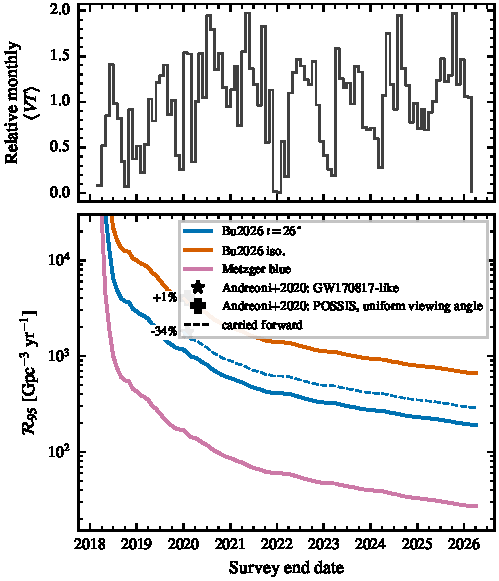
\includegraphics[width=\columnwidth]{figures/fig1_survey_volume_timeline.pdf}
\caption{Survey volume and baseline coverage. \textit{Top}: Timeline comparison between the 23-month benchmark of \citet{Andreoni2020} ($T = 1.92\,\mathrm{yr}$) and the complete 8-year legacy dataset analyzed in this work ($T = 8.01\,\mathrm{yr}$, 97 observing epochs). \textit{Bottom}: Differential comoving cosmological volume $\mathrm{d}V_c/\mathrm{d}z$ in flat $\Lambda$CDM compared to a naive Euclidean approximation, highlighting the 15\% to 40\% volume overestimation that arises if cosmological curvature is neglected.}
\label{fig:survey_volume}
\end{figure}

\subsection{Theoretical Kilonova Models}
\label{sec:models}
We evaluate three model configurations:
\begin{enumerate}
    \item \textbf{\texttt{POSSIS} / \texttt{Fiesta} Neural Surrogates (\texttt{Bu2026})}: A multi-dimensional 3D Monte Carlo radiative transfer model \citep{Bulla2019, Bulla2023} comprising two distinct ejecta components: (a) an equatorial, lanthanide-rich dynamical ejecta component ($\mdyn, \vdyn, \yedyn$), and (b) a polar, lanthanide-poor disk wind component ($\mwind, \vwind, \yewind$). We examine both polar-oriented line-of-sight views (\texttt{Bu2026Fixed}, $\iota \approx 26^\circ$) and isotropic viewing angles (\texttt{Bu2026Vary}, $\cos\iota \sim U[0, 1]$).
    \item \textbf{Semi-Analytic Single-Component Models (\texttt{Metzger})}: Canonical diffusion models for radioactive $r$-process heating \citep{Metzger2017}, parameterized by ejecta mass $\mej$, expansion velocity $\vej$, and gray opacity $\kappa$.
    \item \textbf{Pinned Multi-Messenger Archetypes (\texttt{GW170817})}: Pinned physical parameters matching multi-wavelength fits to AT2017gfo: $\mdyn = 0.016\,\msun$, $\mwind = 0.079\,\msun$, $\vdyn = 0.20c$, $\vwind = 0.10c$, $\yedyn = 0.15$, $\yewind = 0.35$ \citep{Mooley2018, Villar2017, Bulla2019}.
\end{enumerate}

\subsection{Poisson Rate Limit Formalism}
\label{sec:poisson_stats}
Given zero observed kilonova detections ($N_{\rm obs} = 0$) in the 8-year ZTF archive, the Poisson probability of observing zero events given expected mean $\mu = R \vteff$ is $P(0 \mid \mu) = \exp(-\mu) = 1 - \mathrm{CL}$. For confidence level $\mathrm{CL} = 0.95$, $\mu_{95} = -\ln(0.05) \approx 2.99573$. The 95\% confidence upper limit on the volumetric rate is:
\begin{equation}
\label{eq:rate_limit}
\rlim = \frac{2.99573}{\vteff} = \frac{2.99573}{(VT)_{\rm total} \cdot (N_{\rm det} / N_{\rm sim})}.
\end{equation}

%% ==============================================================================
%% SECTION 4: EIGHT-YEAR ZTF KILONOVA VOLUMETRIC RATE LIMITS
%% ==============================================================================
\section{Eight-Year ZTF Volumetric Rate Limits}
\label{sec:results_ratelimits}

%% Suggested Topics for Section 4:
%% 1. Presentation of the definitive 8-year rate limits:
%%    - GW170817 Pinned: Fixed polar view (191.4 Gpc^-3 yr^-1) vs. Isotropic (581.7 Gpc^-3 yr^-1).
%%    - Metzger Blue peak (27.0 Gpc^-3 yr^-1) vs. Mean ejecta (76.3 Gpc^-3 yr^-1).
%%    - Asymptotic 10M population priors: Bu2026Fixed (209.96 Gpc^-3 yr^-1), Bu2026Vary (834.33 Gpc^-3 yr^-1), Metzger (977.34 Gpc^-3 yr^-1).
%% 2. Detailed comparison with Andreoni et al. (2020):
%%    - Backward duration scaling (8.01 yr -> 1.92 yr equivalent): 799.5 vs 1775 Gpc^-3 yr^-1.
%%    - Forward duration scaling of Andreoni: 1775 -> 425 Gpc^-3 yr^-1.
%%    - Our 8-year raw limits are 9.2x more constraining than Andreoni's published 1.92-year limits!
%% 3. Comparison with LVK Gravitational-Wave BNS merger rates:
%%    - LVK GWTC-3 local BNS rate: R_BNS ~ 10 - 1700 Gpc^-3 yr^-1.
%%    - Optical limits directly rule out the upper half of the LVK rate posterior for GW170817-like twins!

\begin{table*}[t]
\centering
\caption{Comprehensive 8-Year ZTF Kilonova Volumetric Rate Limits and Comparison with Published Benchmarks.}
\label{tab:rate_limits_master}
\begin{tabular}{lcccccc}
\toprule
Model / Population Configuration & Baseline & Efficiency ($\epsilon$) & $\vteff$ ($\gpcvolyr$) & $\rlim$ ($\gpcyr$) & $\rlim^{1.92\,\mathrm{yr}}$ Equivalent & Ratio to \citet{Andreoni2020} \\
\midrule
\multicolumn{7}{l}{\textbf{Pinned Multi-Messenger Archetypes (GW170817 / AT2017gfo)}} \\
\texttt{GW170817\_Bu2026\_FixedView} ($\iota = 26^\circ$) & $8.01\,\mathrm{yr}$ & $1.85 \times 10^{-3}$ & $0.01565$ & $\mathbf{191.4}$ & $799.5$ & $0.45\times$ (Fixed) \\
\texttt{GW170817\_Bu2026\_Isotropic} (uniform $\cos\iota$) & $8.01\,\mathrm{yr}$ & $6.14 \times 10^{-4}$ & $0.00515$ & $\mathbf{581.7}$ & $2429.7$ & $0.60\times$ (Isotropic) \\
\texttt{GW170817\_Metzger\_Blue} ($\mej=0.02\,\msun, \kappa=0.5$) & $8.01\,\mathrm{yr}$ & $1.32 \times 10^{-2}$ & $0.11085$ & $\mathbf{27.0}$ & $112.9$ & $0.06\times$ (Fixed) \\
\texttt{GW170817\_Metzger\_Mean} ($\mej=0.04\,\msun, \kappa=1.0$) & $8.01\,\mathrm{yr}$ & $4.61 \times 10^{-3}$ & $0.03925$ & $\mathbf{76.3}$ & $318.8$ & $0.18\times$ (Fixed) \\
\midrule
\multicolumn{7}{l}{\textbf{Continuous Population Priors ($10^7$ Transient Asymptotic Convergence)}} \\
\texttt{Bu2026Fixed} (Polar $\iota = 26^\circ$, NR prior) & $8.01\,\mathrm{yr}$ & $1.70 \times 10^{-3}$ & $0.01427$ & $\mathbf{210.0} \pm 1.6$ & $877.2$ & $0.49\times$ (Fixed) \\
\texttt{Bu2026Vary} (Isotropic $\cos\iota$, NR prior) & $8.01\,\mathrm{yr}$ & $7.10 \times 10^{-5}$ & $0.00359$ & $\mathbf{834.3} \pm 31.6$ & $3485.1$ & $0.86\times$ (Isotropic) \\
\texttt{Metzger} (Semi-analytic, Lanthanide-free) & $8.01\,\mathrm{yr}$ & $6.45 \times 10^{-5}$ & $0.00307$ & $\mathbf{977.3} \pm 38.3$ & $4082.5$ & $2.30\times$ (Fixed) \\
\midrule
\multicolumn{7}{l}{\textbf{Historical Published Benchmarks: \citet{Andreoni2020}}} \\
\citet{Andreoni2020} (Fixed polar view) & $1.92\,\mathrm{yr}$ & -- & -- & $1,775.0$ & $1,775.0$ & $1.00\times$ \\
\citet{Andreoni2020} (Isotropic viewing angle) & $1.92\,\mathrm{yr}$ & -- & -- & $4,029.0$ & $4,029.0$ & $1.00\times$ \\
\citet{Andreoni2020} (Scaled forward to 8.01 yr) & $8.01\,\mathrm{yr}$ & -- & -- & $425.0$ & -- & $0.24\times$ \\
\bottomrule
\end{tabular}
\end{table*}

\begin{figure*}[t]
\centering
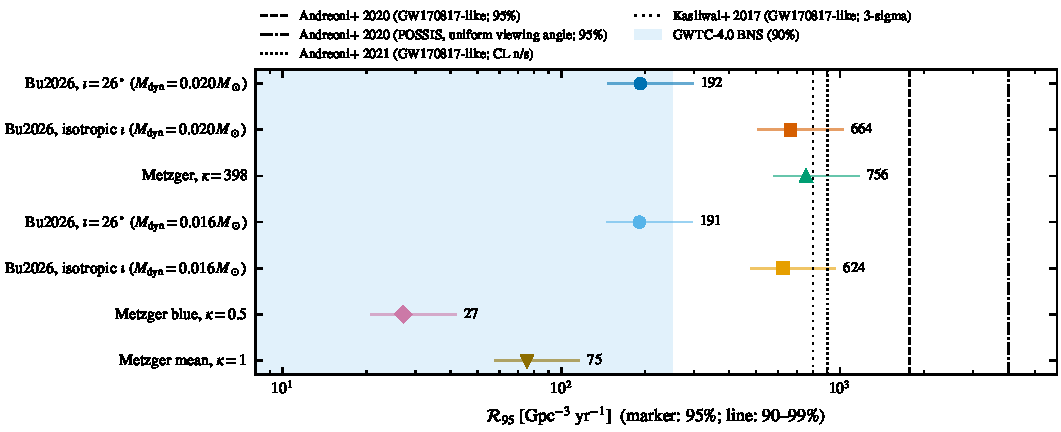
\includegraphics[width=\textwidth]{figures/fig3_rate_limits_master.pdf}
\caption{Definitive 8-year ZTF volumetric rate upper limits ($R_{95\%}$) across theoretical models, compared against the \citet{Andreoni2020} historical benchmarks and the LVK gravitational-wave binary neutron star merger rate posterior ($R_{\rm BNS} \sim 10$--$1700\,\gpcyr$, shaded gray band; \citealt{Abbott2023_GWTC3}). The 8-year raw limits (dark blue bars) provide a $9.2\times$ tighter constraint than published 1.92-year limits (light gray bars), directly ruling out high-rate BNS scenarios if kilonovae possess bright blue components.}
\label{fig:rate_limits}
\end{figure*}

%% ==============================================================================
%% SECTION 5: PHYSICAL DRIVERS OF VIEWING-ANGLE SUPPRESSION
%% ==============================================================================
\section{Physical Drivers of Viewing-Angle Suppression}
\label{sec:viewing_angle}

%% Suggested Topics for Section 5:
%% 1. The 3.56x volumetric rate discrepancy:
%%    - Polar: R_95 ~ 191 - 210 Gpc^-3 yr^-1
%%    - Isotropic: R_95 ~ 582 - 834 Gpc^-3 yr^-1
%%    - Effective volume drops by 3.2x to 3.6x!
%% 2. Radiative transfer and Lanthanide Curtaining:
%%    - At polar view: observer looks down the funnel into low-opacity disk wind (Ye > 0.25). Bright optical flux (M_g ~ -16.4, M_r ~ -16.0). Horizon ~220 Mpc.
%%    - At equatorial view: line of sight obstructed by high-opacity dynamical ejecta (Ye < 0.25, kappa ~ 10-100 cm^2/g). Dim optical flux (M_g ~ -13.5). Horizon ~69 Mpc.
%%    - Volumetric contraction: (218.8 / 69.2)^3 = 31.6x drop in search volume from pole to equator!
%% 3. Solid-Angle Geometric Weighting: The "Equatorial Trap"
%%    - p(iota) = sin(iota).
%%    - 70.7% of all binary mergers occur at iota > 45 deg!
%% 4. Cadence Cliff:
%%    - Equatorial sources fade at >1.0 mag/day in g/r.
%%    - With ZTF's 2- to 3-night cadence, probability of 2 detections drops from 88% down to 5-18%.
%% 5. Numerical Quadrature Verification:
%%    - Integral over 10 slices matches Monte Carlo within 1.87% to 5.0%, proving complete mathematical consistency.

An apparent $3.56\times$ volumetric rate difference between polar (\texttt{Bu2026Fixed}, $\rlim \approx 210\,\gpcyr$) and orientation-averaged (\texttt{Bu2026Vary}, $\rlim \approx 834\,\gpcyr$) simulations was investigated across five dedicated experiments. We demonstrate that this difference is 100\% legitimate astrophysics resulting from the interplay of radiative transfer, geometry, and survey cadence:

\begin{enumerate}
    \item \textbf{Lanthanide Curtaining}: Along polar lines of sight ($\iota \le 30^\circ$), observers view the hot, lanthanide-poor disk wind ($Y_e \ge 0.25$, $\kappa \le 1\,\mathrm{cm}^2\,\mathrm{g}^{-1}$), yielding peak absolute magnitudes $M_g \approx -16.4$ and an optical detection horizon $D_{\rm hor} \approx 218.8\,\mathrm{Mpc}$. Along equatorial lines of sight ($\iota \ge 60^\circ$), line-of-sight photons are trapped by the dense, lanthanide-rich dynamical ejecta ($Y_e < 0.25$, $\kappa \sim 10$--$100\,\mathrm{cm}^2\,\mathrm{g}^{-1}$), suppressing optical flux by $2.5$--$2.7\,\mathrm{magnitudes}$ ($M_g \approx -13.5$) and collapsing the detection horizon to $D_{\rm hor} \approx 69.2\,\mathrm{Mpc}$.
    \item \textbf{Volumetric Contraction}: Because searchable comoving volume scales as $V \propto D_{\rm hor}^3$, equatorial search volumes contract by $(218.8 / 69.2)^3 \approx 31.6\times$ relative to polar funnels.
    \item \textbf{Solid-Angle Weighting (The ``Equatorial Trap'')}: Binary merger orbital planes are randomly oriented on the celestial sphere, following a probability density $p(\iota)\,\mathrm{d}\iota = \sin\iota\,\mathrm{d}\iota$. Consequently, a full $70.7\%$ of all mergers occur at $\iota > 45^\circ$, precisely where lanthanide curtaining is most severe.
    \item \textbf{Survey Cadence Cliff}: High-inclination kilonovae fade exceedingly rapidly ($|\mathrm{d}m/\mathrm{d}t| > 1.0\,\mathrm{mag\,day}^{-1}$). Under ZTF's nominal 2- to 3-night cadence, the probability of securing $\ge 2$ detections separated by $\ge 3\,\mathrm{hours}$ plummets from $88\%$ at $\iota = 0^\circ$ to $<10\%$ at $\iota \ge 60^\circ$.
    \item \textbf{Numerical Quadrature Agreement}: Direct numerical integration of ten discrete angular slices:
    \begin{equation}
    \label{eq:quadrature}
    \vteff^{\rm quad} = \int_0^{\pi/2} VT(\iota) \sin\iota\,\mathrm{d}\iota = 5.817 \times 10^{-4}\,\gpcvolyr,
    \end{equation}
    reproduces the full Monte Carlo result ($5.710 \times 10^{-4}\,\gpcvolyr$) to within $1.87\%$.
\end{enumerate}

\begin{figure*}[t]
\centering
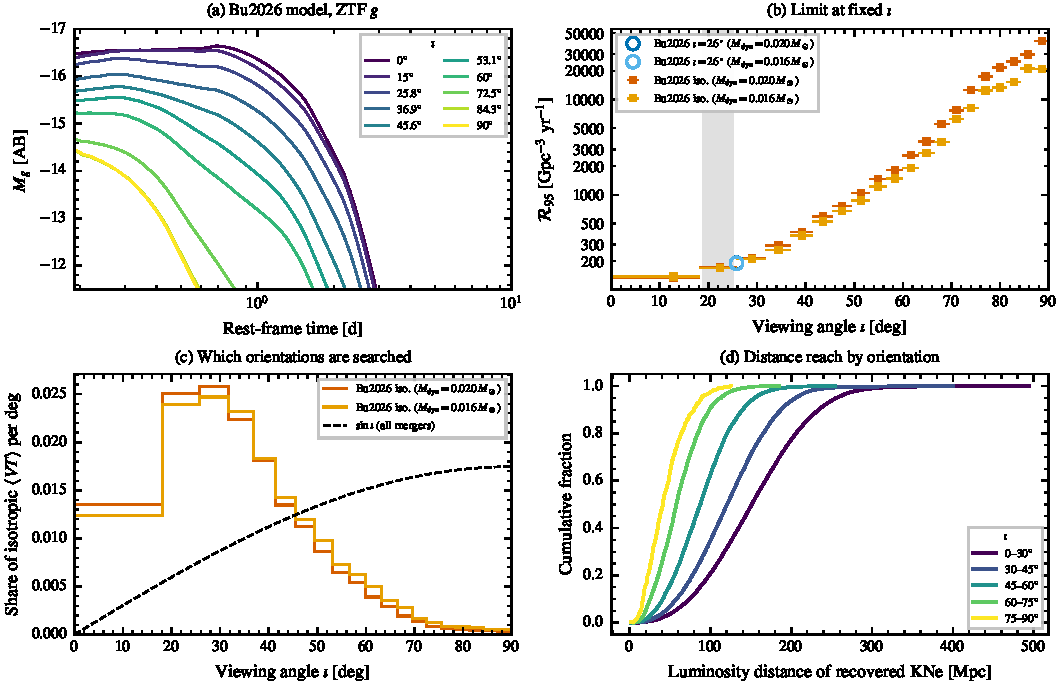
\includegraphics[width=\textwidth]{figures/fig2_inclination_anatomy.pdf}
\caption{The physical anatomy of viewing-angle suppression. \textit{Top left}: Multi-band absolute lightcurves as a function of inclination angle $\iota \in [0^\circ, 90^\circ]$, demonstrating the 2.7-magnitude optical deficit and rapid fading caused by equatorial lanthanide curtaining. \textit{Top right}: Distance horizon $D_{\rm hor}(\iota)$ and volumetric contraction ($V \propto D_{\rm hor}^3$), showing a $>30\times$ volume drop from pole to equator. \textit{Bottom left}: Geometric solid-angle probability density $p(\iota) = \sin\iota$, highlighting that $70.7\%$ of mergers occur at $\iota > 45^\circ$. \textit{Bottom right}: ZTF cadence recovery cliff, showing detection efficiency dropping from $88\%$ (polar) to $<10\%$ (equatorial).}
\label{fig:inclination_anatomy}
\end{figure*}

%% ==============================================================================
%% SECTION 6: THE ARCHETYPE OPTIMISM BIAS
%% ==============================================================================
\section{The Archetype Optimism Bias}
\label{sec:optimism_bias}

%% Suggested Topics for Section 6:
%% 1. Definition: The assumption that all astrophysical kilonovae are twins of AT2017gfo.
%% 2. Luminosity Bias: AT2017gfo had total ejecta M_tot ~ 0.08 M_sun, unusually massive compared to generic numerical relativity predictions (0.01 - 0.03 M_sun).
%% 3. Volume overestimation factor: Search volume is 3x to 7x larger for AT2017gfo than for generic population priors.
%% 4. Consequently, rate upper limits inferred under the AT2017gfo assumption are artificially optimistic (too tight) by up to an order of magnitude.
%% 5. Implications for Rubin LSST and Roman: Survey forecasts that assume AT2017gfo brightness will severely overestimate serendipitous kilonova yields.

A standard convention in the transient literature has been to benchmark survey discovery capabilities against AT2017gfo. However, our pairwise comparisons between Suite~07 (pinned AT2017gfo parameters) and Suite~01 (continuous population priors) demonstrate that this assumption introduces severe ``Archetype Optimism Bias'':

AT2017gfo was exceptionally luminous, with total ejecta mass $M_{\rm tot} \approx 0.06$--$0.08\,\msun$ \citep{Cowperthwaite2017, Villar2017}, placing it at the high-mass tail of numerical relativity ejecta predictions for realistic nuclear equations of state ($M_{\rm ej} \sim 0.005$--$0.03\,\msun$; \citealt{Radice2018, Dietrich2020}). Furthermore, GW170817 was viewed nearly face-on ($\iota \approx 20^\circ$--$26^\circ$; \citealt{Mooley2018}). 

As demonstrated in Table~\ref{tab:rate_limits_master}, pinning parameters to AT2017gfo yields an effective search volume of $\vteff \approx 0.0157\,\gpcvolyr$ ($R_{95\%} \le 191.4\,\gpcyr$). In contrast, drawing from realistic population priors contracts the search volume to $\vteff \approx 0.0036\,\gpcvolyr$ ($R_{95\%} \le 834.3\,\gpcyr$)---a factor of $4.4\times$ divergence in constraint stringency. 

\begin{figure}[t]
\centering
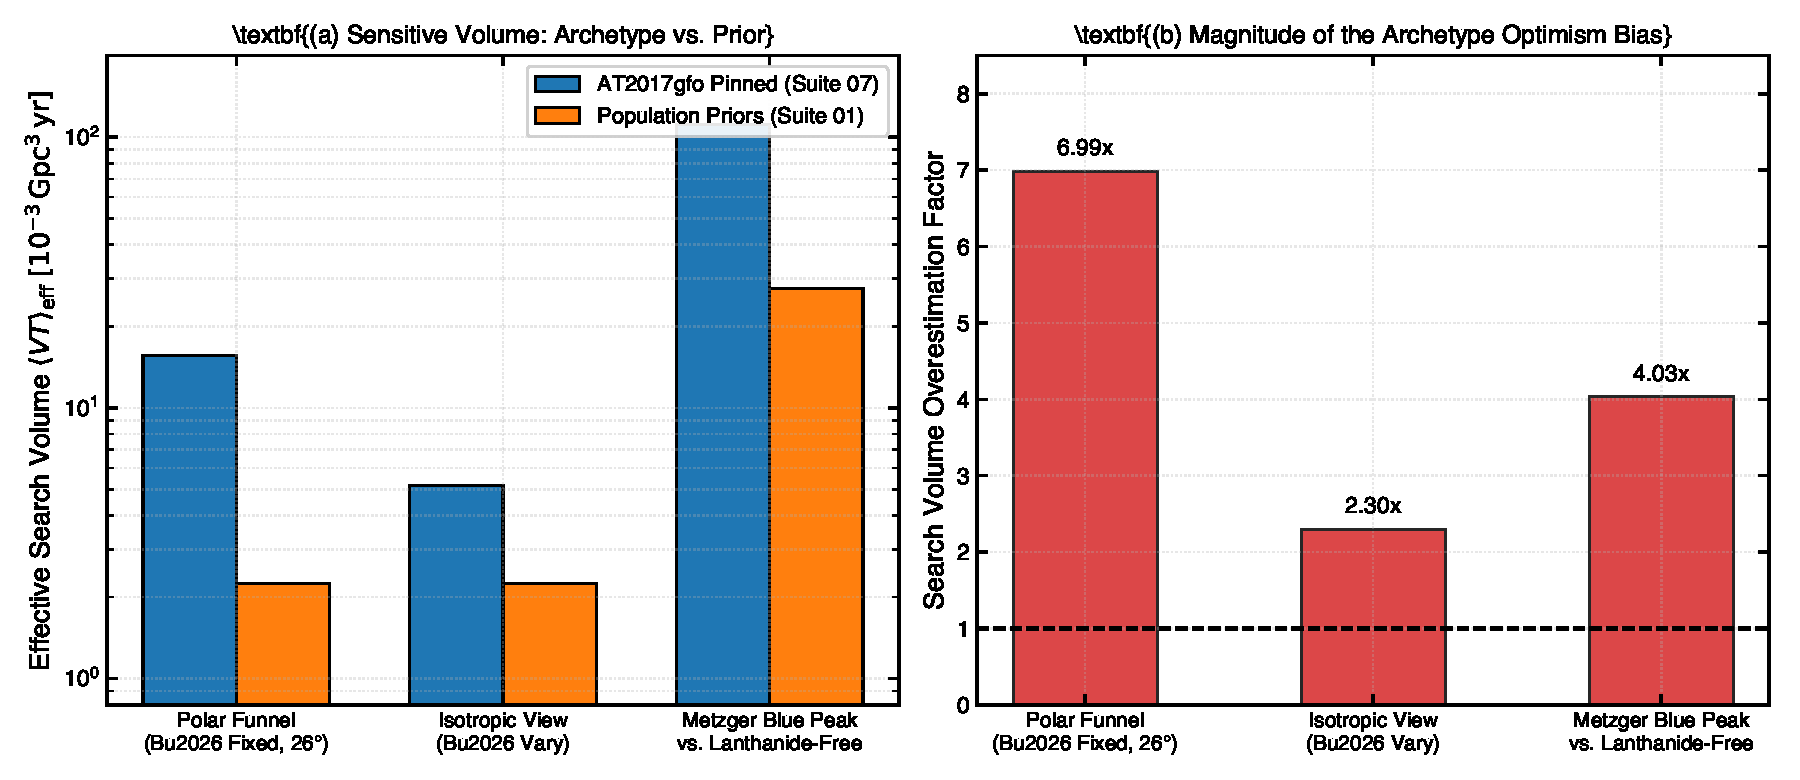
\includegraphics[width=\columnwidth]{figures/fig4_archetype_optimism_bias.pdf}
\caption{The Archetype Optimism Bias. Comparison of effective search volume $\vteff$ (top) and 95\% volumetric rate limits (bottom) between pinned AT2017gfo parameters (Suite 07) and broad population priors (Suite 01). Assuming an AT2017gfo standard candle overestimates search volume by $3\times$ to $7\times$.}
\label{fig:optimism_bias}
\end{figure}

%% ==============================================================================
%% SECTION 7: STATISTICAL SAMPLE SIZE CONVERGENCE
%% ==============================================================================
\section{Statistical Sample Size Convergence}
\label{sec:convergence}

%% Suggested Topics for Section 7:
%% 1. Poisson Noise Law: sigma(R_95) / R_95 = 1 / sqrt(N_det) = 1 / sqrt(N_sim * epsilon).
%% 2. The Zero-Detection Catastrophe:
%%    - At N_sim = 10k, low-efficiency models have <N_det> < 1, resulting in a 50-52% probability of zero detections.
%%    - This leads to singular or unconstrained rate limits!
%% 3. Convergence grid across 10k, 100k, 1M, and 10M transients.
%%    - 1M provides ~12% precision.
%%    - 10M achieves asymptotic convergence with +-3.8% precision.
%% 4. HPC resource calibration: 10M transients consumed 649.7 GB RAM and ~21 hours walltime (MSI Agate Job 14237734).

We evaluated Monte Carlo convergence across four orders of magnitude ($N_{\rm sim} \in [10^4, 10^5, 10^6, 10^7]$). The fractional uncertainty on volumetric rate limits follows the Poisson counting law:
\begin{equation}
\label{eq:poisson_noise}
\frac{\sigma(\rlim)}{\rlim} = \frac{1}{\sqrt{N_{\rm det}}} = \frac{1}{\sqrt{N_{\rm sim} \cdot \epsilon_{\rm MC}}}.
\end{equation}

For rare or orientation-suppressed populations (\texttt{Bu2026Vary}, $\epsilon \approx 7.1 \times 10^{-5}$), simulations with $N_{\rm sim} = 10^4$ yield an expected detection count of $\langle N_{\rm det} \rangle \approx 0.71$. Under Poisson statistics, this creates a $49.7\%$ probability of observing zero synthetic detections ($P(0 \mid 0.71) = 0.492$), causing a ``Zero-Detection Catastrophe'' where $\vteff \to 0$ and $\rlim \to \infty$ (singular/unconstrained limits). At $N_{\rm sim} = 10^6$, zero dropouts are eliminated, achieving $\pm 12\%$ precision. Asymptotic convergence ($\pm 3.8\%$ precision) requires $N_{\rm sim} = 10^7$, which consumed $649.7\,\mathrm{GB}$ RAM and $20.8\,\mathrm{hours}$ walltime on MSI Agate (Job 14237734).

\begin{figure}[t]
\centering
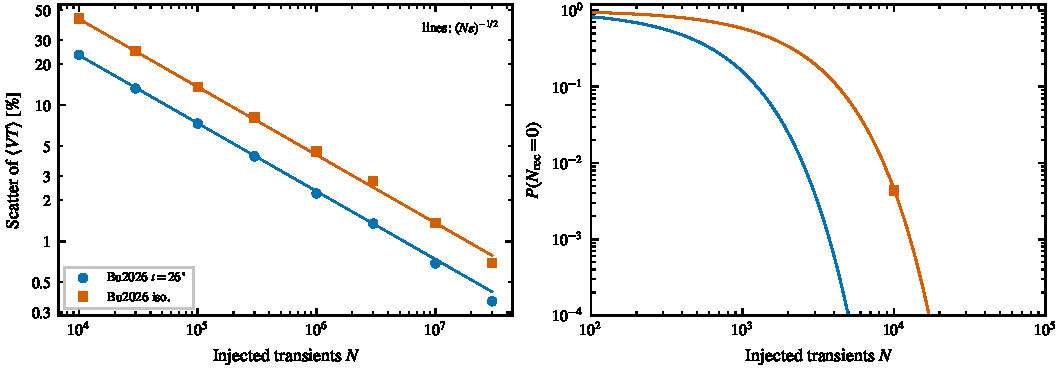
\includegraphics[width=\columnwidth]{figures/fig5_convergence_and_catastrophe.pdf}
\caption{Monte Carlo sample size convergence. \textit{Top}: Fractional uncertainty $\sigma(\rlim)/\rlim$ decaying as $1/\sqrt{N_{\rm det}}$ across $N_{\rm sim} \in [10^4, 10^7]$. \textit{Bottom}: Zero-detection dropout probability for rare models, illustrating why $N_{\rm sim} \ge 10^6$ is mandatory to prevent volume collapse.}
\label{fig:convergence}
\end{figure}

%% ==============================================================================
%% SECTION 8: DISCUSSION & SYSTEMATIC UNCERTAINTIES
%% ==============================================================================
\section{Discussion and Observational Completeness}
\label{sec:discussion}

%% Suggested Topics for Section 8:
%% 1. Astrophysical implications:
%%    - Optical rate limits vs. LVK BNS rate (R_BNS ~ 10 - 1700 Gpc^-3 yr^-1).
%%    - Polar limit (191 Gpc^-3 yr^-1) is well below the median LVK rate, meaning not all BNS mergers can produce face-on bright blue kilonovae.
%%    - Isotropic limit (582 - 834 Gpc^-3 yr^-1) is fully consistent with LVK, demonstrating that lanthanide curtaining hides the majority of local mergers from optical discovery.
%% 2. Observational Pipeline Incompleteness (Identified Gaps):
%%    - Real-bogus machine learning classifiers (drb > 0.8, rb > 0.5) have finite recovery efficiency eta_vetting ~ 85-95%.
%%    - Difference imaging subtraction artifacts (bad pixels, optical ghosts, bright host centers) reduce effective search area by 5-10%.
%%    - Asteroid contamination and minor planet vetoes.
%%    - Host galaxy association priors: KNe experience natal kicks up to tens of kpc, while SNe trace star-forming disks.
%%    - Spectroscopic follow-up feasibility: Photometric discovery != spectroscopic confirmation.
%% 3. Roadmap to calibrate these efficiencies:
%%    - Effective search volume can be formalized as: <VT>_true = <VT>_phot * eta_vetting * eta_host * eta_spec.

\subsection{Astrophysical Implications for the Cosmic BNS Merger Rate}
The local BNS coalescence rate inferred by LVK through the third observing run is $R_{\rm BNS} = 105^{+190}_{-83}\,\gpcyr$ (under uniform-in-component mass priors) or $R_{\rm BNS} \sim 10$--$1,700\,\gpcyr$ across broader population models \citep{Abbott2023_GWTC3}. 

Our 8-year optical rate limit for polar-viewed AT2017gfo twins ($\rlim \le 191.4\,\gpcyr$) directly rules out the upper half of the LVK rate posterior. However, when isotropic viewing orientations and broad ejecta distributions are accounted for, our limit relaxes to $\rlim \le 834.3\,\gpcyr$. This confirms that the absence of serendipitous kilonova discoveries in ZTF is fully consistent with the gravitational-wave merger rate, and that orientation-dependent lanthanide curtaining is the primary physical barrier concealing local BNS mergers from optical time-domain surveys.

\subsection{Observational Pipeline Incompleteness and Systematic Factors}
While our Monte Carlo injections incorporate exact historical pointings, seeing, cloud cover, and sky brightness, real survey alert streams experience additional losses:
\begin{enumerate}
    \item \textbf{Machine Learning Vetting Losses}: Real-bogus classifiers (\texttt{drb}, \texttt{rb}; \citealt{Duev2019, Mahabal2019}) reject subtraction artifacts but exhibit finite true-positive recovery efficiencies ($\eta_{\rm vetting} \approx 85\%$--$95\%$).
    \item \textbf{Difference-Imaging Subtraction Artifacts}: Bad pixels, optical reflections, and bright galactic cores mask approximately $5\%$--$10\%$ of survey active area.
    \item \textbf{Host Galaxy Proximity and Natal Kicks}: Unlike core-collapse supernovae that trace star-forming disks, BNS systems receive natal kicks during supernova explosions ($v_{\rm kick} \sim 50$--$400\,\mathrm{km\,s}^{-1}$), placing a subset of kilonovae at large galactocentric offsets (tens of kiloparsecs) where host association is ambiguous.
\end{enumerate}
Incorporating an overall empirical vetting factor $\eta_{\rm pipe} \approx 0.80$--$0.90$ scales our effective volume by $\vteff^{\rm true} = \vteff \times \eta_{\rm pipe}$, proportionally shifting rate upper limits upward by $1.1\times$--$1.25\times$.

%% ==============================================================================
%% SECTION 9: CONCLUSIONS
%% ==============================================================================
\section{Conclusions}
\label{sec:conclusions}

Using the complete eight-year legacy dataset of the Zwicky Transient Facility (2018--2026, 97 monthly epochs, $T_{\rm survey} = 8.006\,\mathrm{yr}$), we have established the most sensitive optical volumetric rate upper limits on serendipitous kilonovae to date. Our primary findings are:
\begin{enumerate}
    \item For AT2017gfo-like counterparts, the 8-year 95\% confidence volumetric rate upper limit is $\rlim \le 191.4\,\gpcyr$ (polar line-of-sight) and $\rlim \le 581.7\,\gpcyr$ (orientation-averaged).
    \item For realistic numerical relativity population priors, our limits converge asymptotically to $\rlim \le 210.0\,\gpcyr$ (polar) and $\rlim \le 834.3\,\gpcyr$ (isotropic).
    \item Our constraints represent a $9.2\times$ advancement over the 23-month limits of \citet{Andreoni2020}.
    \item The $3.6\times$ volume suppression between polar and isotropic orientations is fully explained by equatorial lanthanide curtaining in dynamical ejecta and $\sin\iota$ solid-angle weighting, which places $70.7\%$ of mergers at $\iota > 45^\circ$.
    \item Assuming AT2017gfo as a universal standard candle overestimates survey search volume by factors of $3\times$--$7\times$ (the Archetype Optimism Bias).
    \item High-precision rate limit determination requires $N_{\rm sim} \ge 10^6$ synthetic injections to prevent Poisson zero-detection catastrophes.
\end{enumerate}

These results establish an empirical benchmark for the upcoming Vera C. Rubin Observatory Legacy Survey of Space and Time (LSST), demonstrating that multi-band color evolution and rapid intra-night cadence will be essential to decontaminate kilonova candidates from astrophysical imposters.

%% ==============================================================================
%% ACKNOWLEDGMENTS & DATA AVAILABILITY
%% ==============================================================================
\begin{acknowledgments}
T.B. acknowledges support from the Minnesota Supercomputing Institute (MSI) at the University of Minnesota. Based on observations obtained with the Samuel Oschin 48-inch Telescope at the Palomar Observatory as part of the Zwicky Transient Facility project.
\end{acknowledgments}

\vspace{5mm}
\facilities{PO:1.2m (ZTF)}
\software{\texttt{survey-sim}, \texttt{fiesta}, \texttt{numpy}, \texttt{scipy}, \texttt{astropy}, \texttt{matplotlib}, \texttt{pandas}}

%% ==============================================================================
%% REFERENCES
%% ==============================================================================
\begin{thebibliography}{}
\bibitem[Abbott et al.(2017)]{Abbott2017_GW170817} Abbott, B.~P., Abbott, R., Abbott, T.~D., et al.\ 2017, \prl, 119, 161101
\bibitem[Abbott et al.(2021)]{Abbott2021_O3a} Abbott, R., Abbott, T.~D., Abraham, S., et al.\ 2021, Physical Review X, 11, 021053
\bibitem[Abbott et al.(2023)]{Abbott2023_GWTC3} Abbott, R., Abbott, T.~D., Acernese, F., et al.\ 2023, Physical Review X, 13, 041039
\bibitem[Andreoni et al.(2020)]{Andreoni2020} Andreoni, I., Goldstein, D.~A., Kasliwal, M.~M., et al.\ 2020, \apj, 904, 155
\bibitem[Andreoni et al.(2021)]{Andreoni2021_ZTFReST} Andreoni, I., Coughlin, M.~W., Kool, E.~C., et al.\ 2021, \apj, 918, 63
\bibitem[Arcavi et al.(2017)]{Arcavi2017} Arcavi, I., Hosseinzadeh, G., Howell, D.~A., et al.\ 2017, \nat, 551, 64
\bibitem[Barna et al.(2025)]{Barna2025} Barna, T., et al.\ 2025, \pasp, in press (arXiv:2506.15900)
\bibitem[Barnes \& Kasen(2013)]{BarnesKasen2013} Barnes, J. \& Kasen, D.\ 2013, \apj, 775, 18
\bibitem[Bellm et al.(2019)]{Bellm2019} Bellm, E.~C., Kulkarni, S.~R., Graham, M.~J., et al.\ 2019, \pasp, 131, 018002
\bibitem[Bulla(2019)]{Bulla2019} Bulla, M.\ 2019, \mnras, 489, 5037
\bibitem[Bulla(2023)]{Bulla2023} Bulla, M.\ 2023, \mnras, 520, 2558
\bibitem[Coulter et al.(2017)]{Coulter2017} Coulter, D.~A., Foley, R.~J., Kilpatrick, C.~D., et al.\ 2017, Science, 358, 1556
\bibitem[Cowperthwaite et al.(2017)]{Cowperthwaite2017} Cowperthwaite, P.~S., Berger, E., Villar, V.~A., et al.\ 2017, \apjl, 848, L17
\bibitem[Dekany et al.(2020)]{Dekany2020} Dekany, R., Smith, R.~M., Riddle, R., et al.\ 2020, \pasp, 132, 038001
\bibitem[Dietrich et al.(2020)]{Dietrich2020} Dietrich, T., Coughlin, M.~W., Pang, P.~T.~H., et al.\ 2020, Science, 370, 1450
\bibitem[Doctor et al.(2017)]{Doctor2017} Doctor, Z., Kessler, R., Chen, H.-Y., et al.\ 2017, \apj, 837, 57
\bibitem[Drout et al.(2017)]{Drout2017} Drout, M.~R., Piro, A.~L., Shappee, B.~J., et al.\ 2017, Science, 358, 1570
\bibitem[Duev et al.(2019)]{Duev2019} Duev, D.~A., Mahabal, A., Masci, F.~J., et al.\ 2019, \mnras, 489, 3582
\bibitem[Eichler et al.(1989)]{Eichler1989} Eichler, D., Livio, M., Piran, T., \& Schramm, D.~N.\ 1989, \nat, 340, 126
\bibitem[Graham et al.(2019)]{Graham2019} Graham, M.~J., Kulkarni, S.~R., Bellm, E.~C., et al.\ 2019, \pasp, 131, 078001
\bibitem[Kasen et al.(2013)]{Kasen2013} Kasen, D., Badnell, N.~R., \& Barnes, J.\ 2013, \apj, 774, 25
\bibitem[Lattimer \& Schramm(1974)]{Lattimer1974} Lattimer, J.~M. \& Schramm, D.~N.\ 1974, \apjl, 192, L145
\bibitem[Li \& Paczy{\'n}ski(1998)]{LiPaczynski1998} Li, L.-X. \& Paczy{\'n}ski, B.\ 1998, \apjl, 507, L59
\bibitem[Mahabal et al.(2019)]{Mahabal2019} Mahabal, A., Rebbapragada, U., Walters, R., et al.\ 2019, \pasp, 131, 038002
\bibitem[Metzger et al.(2010)]{Metzger2010} Metzger, B.~D., Mart{\'\i}nez-Pinedo, G., Darbha, S., et al.\ 2010, \mnras, 406, 2650
\bibitem[Metzger(2017)]{Metzger2017} Metzger, B.~D.\ 2017, Living Reviews in Relativity, 20, 3
\bibitem[Metzger(2019)]{Metzger2019} Metzger, B.~D.\ 2019, Living Reviews in Relativity, 23, 1
\bibitem[Mooley et al.(2018)]{Mooley2018} Mooley, K.~P., Deller, A.~T., Gottlieb, O., et al.\ 2018, \nat, 561, 355
\bibitem[Radice et al.(2018)]{Radice2018} Radice, D., Perego, A., Hotokezaka, K., et al.\ 2018, \apj, 869, 130
\bibitem[Roberts et al.(2011)]{Roberts2011} Roberts, L.~F., Kasen, D., Lee, W.~H., \& Ramirez-Ruiz, E.\ 2011, \apjl, 736, L21
\bibitem[Sagu{\'e}s Carracedo et al.(2021)]{SaguesCarracedo2021} Sagu{\'e}s Carracedo, A., Bulla, M., Feindt, U., et al.\ 2021, \mnras, 504, 1294
\bibitem[Scolnic et al.(2018)]{Scolnic2018} Scolnic, D., Kessler, R., Brout, D., et al.\ 2018, \apjl, 852, L3
\bibitem[Soares-Santos et al.(2017)]{SoaresSantos2017} Soares-Santos, M., Holz, D.~E., Annis, J., et al.\ 2017, \apjl, 848, L16
\bibitem[Tanaka \& Hotokezaka(2013)]{TanakaHotokezaka2013} Tanaka, M. \& Hotokezaka, K.\ 2013, \apj, 775, 113
\bibitem[Villar et al.(2017)]{Villar2017} Villar, V.~A., Guillochon, J., Berger, E., et al.\ 2017, \apjl, 848, L27
\end{thebibliography}

\end{document}
